% ============================================================
%  Supplementary Material
%  "A Controlled Synthetic Sentinel-2 L1C Benchmark for
%   Methane Plume Segmentation"
%
%  Compile standalone on Overleaf:
%    pdflatex supplement  (no bibtex pass needed)
% ============================================================
\documentclass[10pt,letterpaper]{article}

% --- geometry & layout ------------------------------------------
\usepackage[letterpaper,
            top=2.5cm, bottom=2.5cm,
            left=2cm,  right=2cm]{geometry}
\usepackage{multicol}          % for optional two-column body

% --- graphics & color -------------------------------------------
\usepackage{graphicx}
\usepackage[dvipsnames,svgnames,x11names]{xcolor}

% --- fonts & encoding -------------------------------------------
\usepackage[T1]{fontenc}
\usepackage[utf8]{inputenc}
\usepackage[protrusion=true,expansion=false]{microtype}

% --- math -------------------------------------------------------
\usepackage{amsmath,amssymb}

% --- tables -----------------------------------------------------
\usepackage{booktabs}
\usepackage{array}

% --- hyperref ---------------------------------------------------
\usepackage[colorlinks=true,
            linkcolor=NavyBlue,
            citecolor=NavyBlue,
            urlcolor=NavyBlue]{hyperref}

% --- caption formatting ----------------------------------------
\usepackage[labelfont=bf,
            labelsep=period,
            font=small]{caption}

% --- header / footer -------------------------------------------
\usepackage{fancyhdr}
\pagestyle{fancy}
\fancyhf{}
\renewcommand{\headrulewidth}{0.4pt}
\lhead{\small\textit{Supplementary Material}}
\rhead{\small\textit{CH\textsubscript{4} Plume Segmentation Benchmark}}
\cfoot{\small\thepage}

% --- figure counter: S1, S2, … ---------------------------------
\renewcommand{\thefigure}{S\arabic{figure}}
\renewcommand{\thetable}{S\arabic{table}}
\renewcommand{\theequation}{S\arabic{equation}}

% ================================================================
\begin{document}

% ----------------------------------------------------------------
%  Title block
% ----------------------------------------------------------------
\begin{center}
  {\Large\bfseries Supplementary Material}\\[0.6em]
  {\large A Controlled Synthetic Sentinel-2 L1C Benchmark\\
         for Methane Plume Segmentation}\\[1.0em]
  {\normalsize
   \textit{This document accompanies the main article and provides
   five additional qualitative prediction examples (Figures~S1--S5)
   not shown in the main text.}}
\end{center}

\vspace{0.5em}
\noindent\rule{\linewidth}{0.6pt}
\vspace{0.5em}

% ----------------------------------------------------------------
%  Introduction paragraph
% ----------------------------------------------------------------
\noindent
Figure~1 of the main paper shows a single representative qualitative
comparison between the five benchmarked architectures
(U-Net, Attention U-Net, U-Net++, DeepLabV3+, and PhysTAUNet) on a
held-out synthetic TEST patch.  Here we provide five additional
examples (Figures~S1--S5) drawn from the same held-out TEST split,
selected to illustrate a range of plume morphologies, optical depths,
and background landscapes.

Specifically, each panel shows, from left to right: the RGB composite
of the Sentinel-2 L1C background chip (Bands~4, 3, 2); the SWIR ratio
delta $\Delta r$ used as the primary detection feature; the
ground-truth soft plume mask (i.e., the physics-informed Beer--Lambert
attenuation target); and the predicted probability maps produced by
each of the five models after thresholding at $0.5$.  All inputs are
from background chips not used during training or checkpoint selection,
and all plume fields were generated by the same synthetic injection
procedure described in Section~3 of the main text.

Across examples, we observe that all models consistently localize the
dense plume core but diverge most at the diffuse, low-optical-depth
periphery and at detached wisp structures, in agreement with the
systematic gap between strict and tolerant F1 scores reported in
Table~1 of the main paper.  DeepLabV3+ tends to produce the most
conservative probability maps (high precision, lower recall), while
U-Net tends toward the most expansive responses (lower precision,
higher recall).  Attention U-Net's gating mechanism yields the most
calibrated predicted extents across these examples, consistent with
its leading position in Table~1.  PhysTAUNet's auxiliary
$\tau_0$-regression head does not translate into a systematic visual
advantage over the simpler baselines in these examples, corroborating
the quantitative findings.

\vspace{0.8em}
\noindent\rule{\linewidth}{0.4pt}

% ================================================================
%  Qualitative figures S1 -- S5
% ================================================================

% --- Figure S1 --------------------------------------------------
\begin{figure*}[!htb]
  \centering
  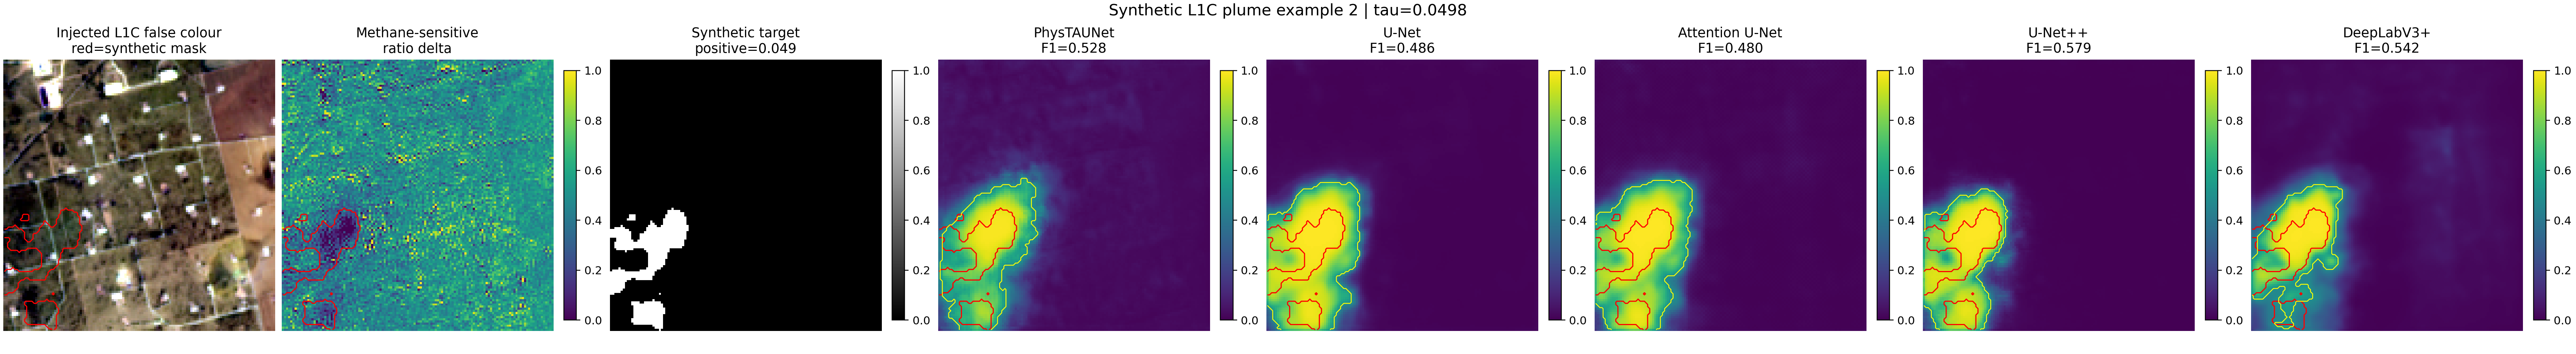
\includegraphics[width=\linewidth]{figures/synthetic_example_02_model_comparison.png}
  \caption{%
    \textbf{Qualitative example S1.}  Held-out synthetic TEST patch.
    From left to right: RGB composite (Bands~4--3--2), SWIR ratio
    delta $\Delta r$, ground-truth soft target, and predicted
    probability maps for U-Net, Attention U-Net, U-Net++,
    DeepLabV3+, and PhysTAUNet.  This example features a compact,
    high-optical-depth plume core over a mixed agricultural--bare-soil
    background.  All models correctly detect the core; disagreement is
    concentrated at the diffuse periphery.
  }
  \label{fig:S1}
\end{figure*}


% --- Figure S2 --------------------------------------------------
\begin{figure*}[!htb]
  \centering
  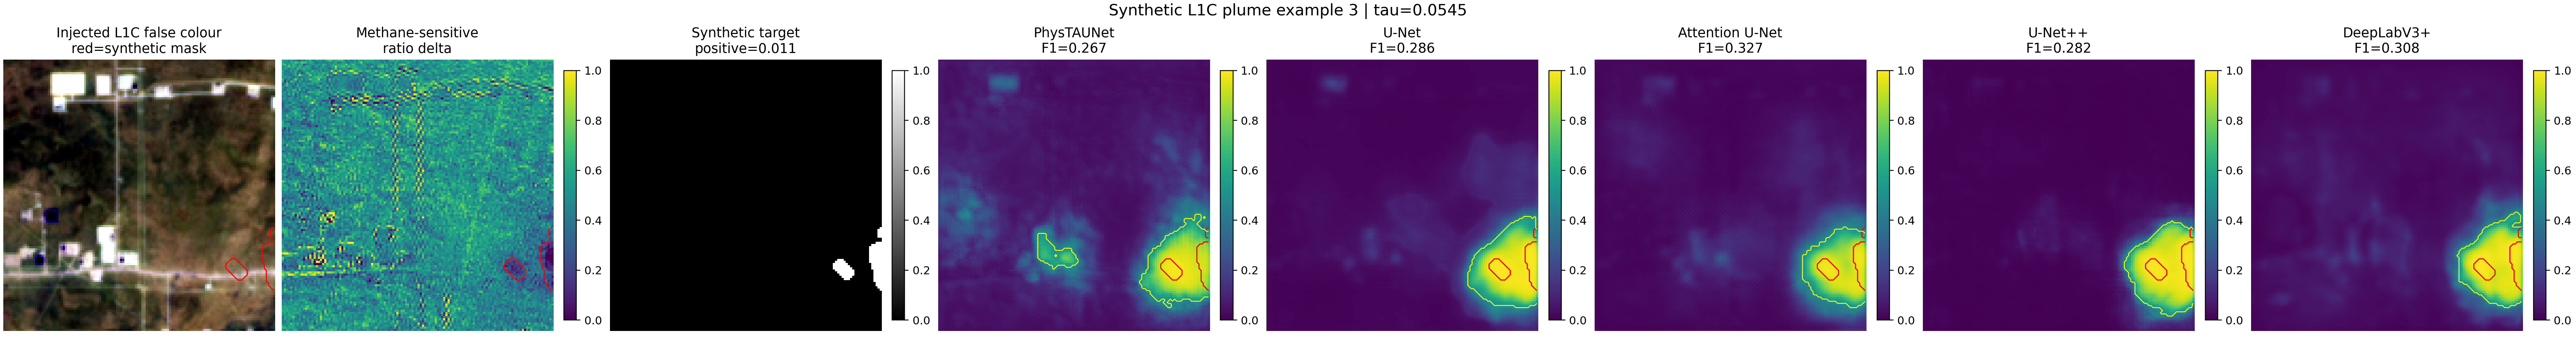
\includegraphics[width=\linewidth]{figures/synthetic_example_03_model_comparison.png}
  \caption{%
    \textbf{Qualitative example S2.}  Held-out synthetic TEST patch.
    This example exhibits an elongated, wind-streaked plume morphology
    with lower peak optical depth ($\tau_0 < 0.05$).  Detection
    difficulty is elevated relative to Fig.~S1: U-Net and Attention
    U-Net recover the elongated tail more reliably than DeepLabV3+,
    whose conservative decision boundary suppresses the low-response
    tail region.  PhysTAUNet's $\tau_0$ auxiliary output does not
    provide a clear advantage over Attention U-Net on this example.
  }
  \label{fig:S2}
\end{figure*}


% --- Figure S3 --------------------------------------------------
\begin{figure*}[!htb]
  \centering
  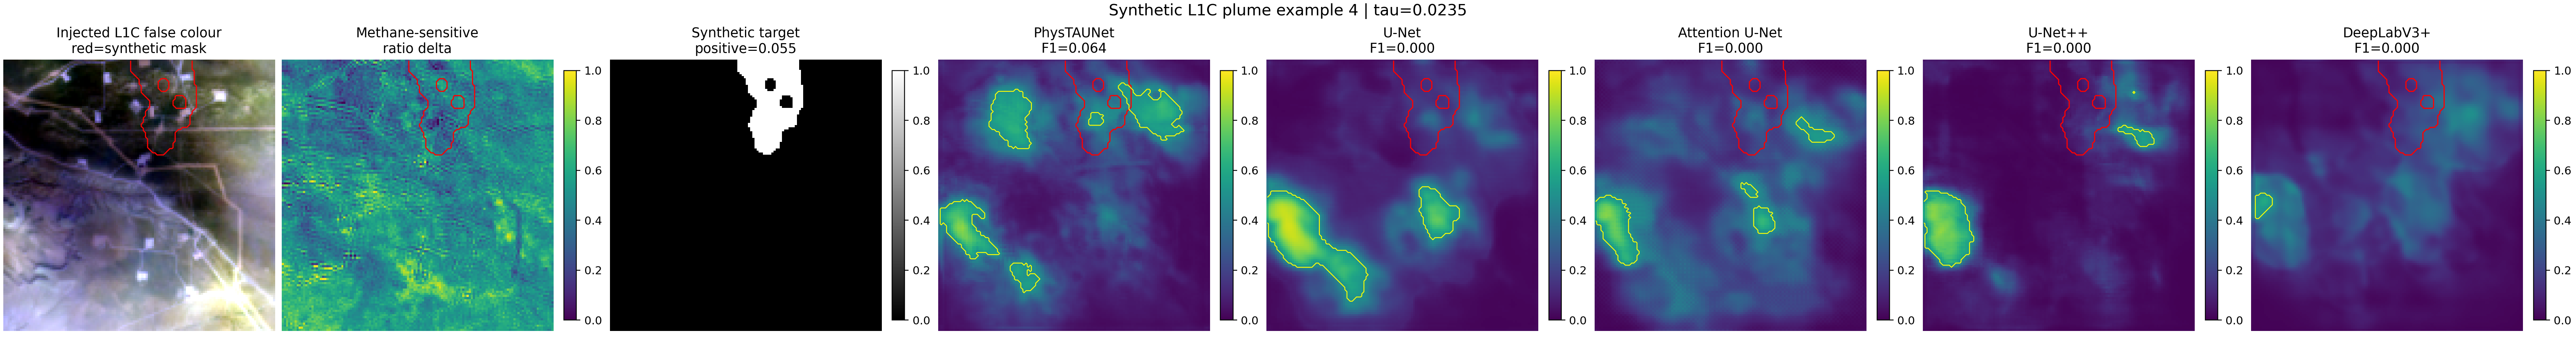
\includegraphics[width=\linewidth]{figures/synthetic_example_04_model_comparison.png}
  \caption{%
    \textbf{Qualitative example S3.}  Held-out synthetic TEST patch.
    This patch contains a spatially fragmented plume (i.e., a main
    lobe with at least one detached wisp region) over heterogeneous
    terrain.  The detached wisp (lower right quadrant of the target
    mask) is missed by all five models, demonstrating a shared failure
    mode rather than an architecture-specific one.  The main lobe is
    recovered by all models.
  }
  \label{fig:S3}
\end{figure*}


% --- Figure S4 --------------------------------------------------
\begin{figure*}[!htb]
  \centering
  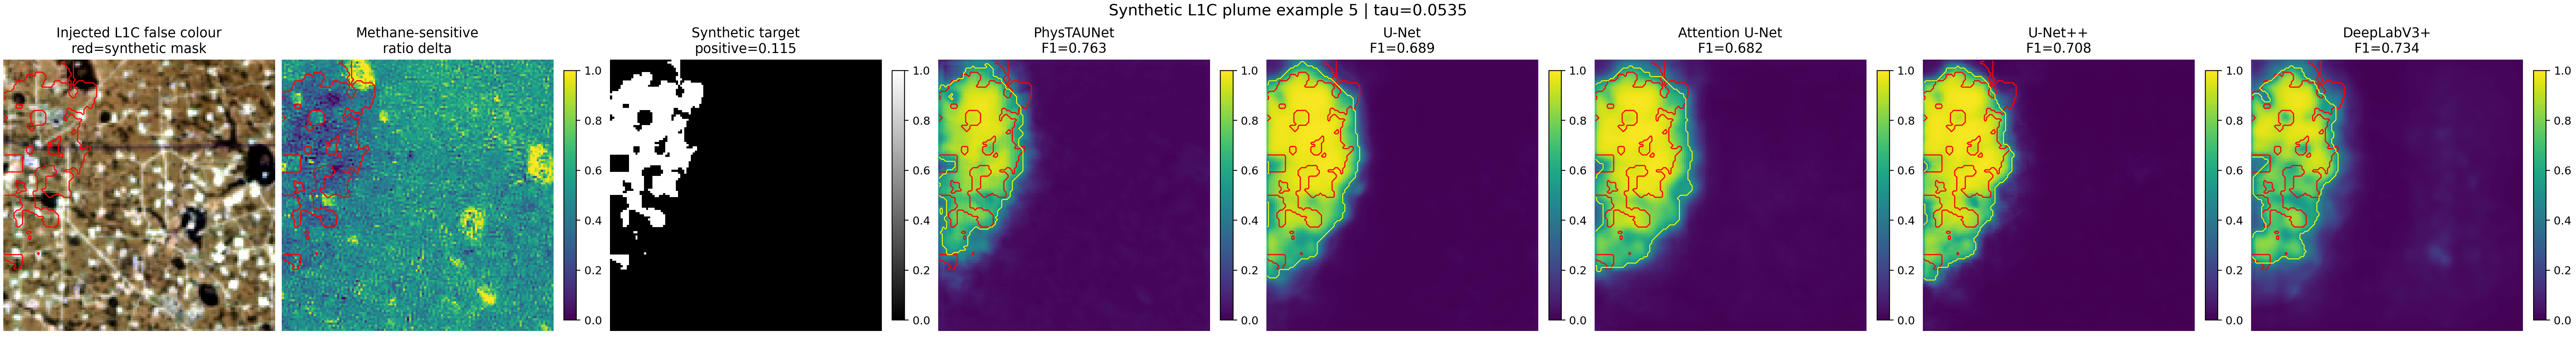
\includegraphics[width=\linewidth]{figures/synthetic_example_05_model_comparison.png}
  \caption{%
    \textbf{Qualitative example S4.}  Held-out synthetic TEST patch.
    This example shows a plume injected over a vegetation-dominated
    background (high NDVI), where the SWIR signal contrast is moderate
    but the RGB composite provides little visual cue.  U-Net++
    produces a noticeably noisier probability map than the other four
    models on this background type, consistent with its lower TEST F1
    reported in Table~1.
  }
  \label{fig:S4}
\end{figure*}


% --- Figure S5 --------------------------------------------------
\begin{figure*}[!htb]
  \centering
  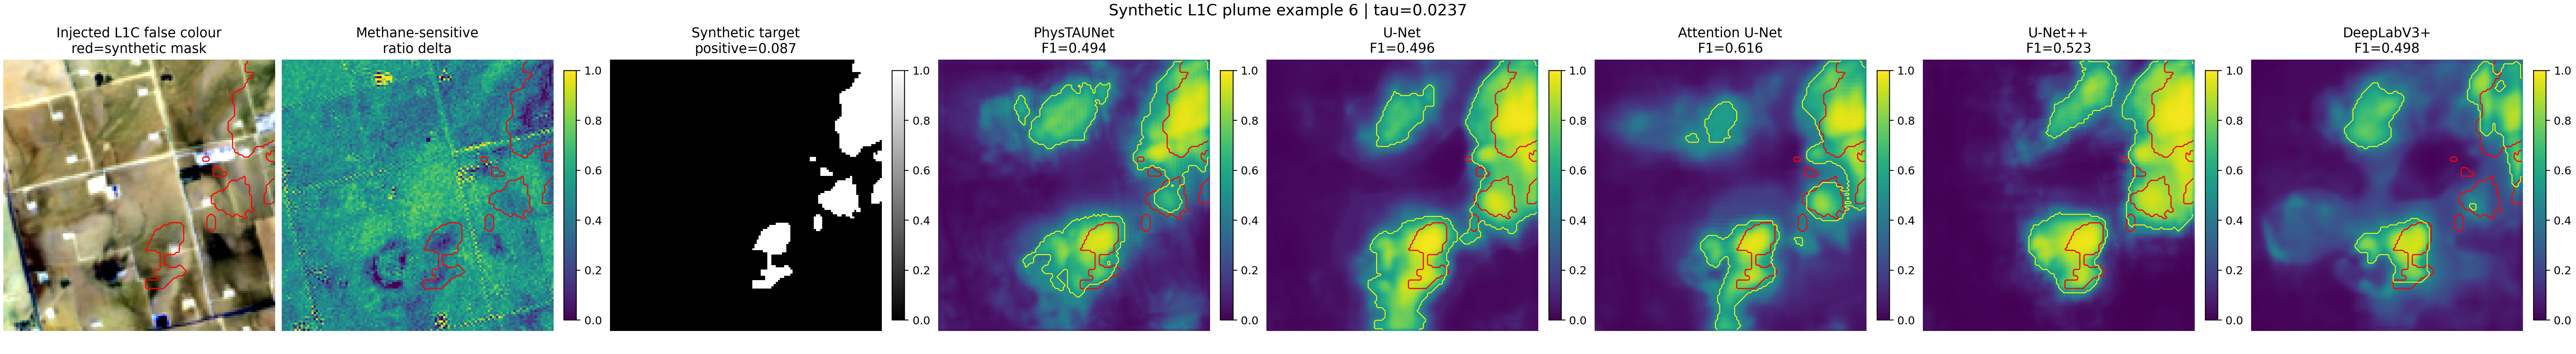
\includegraphics[width=\linewidth]{figures/synthetic_example_06_model_comparison.png}
  \caption{%
    \textbf{Qualitative example S5.}  Held-out synthetic TEST patch.
    A large-area, high-optical-depth plume over a predominantly bare
    or low-vegetation background.  On examples such as this one
    (where the plume is large and the SWIR contrast is strong), all
    five models achieve near-complete recall and their probability
    maps are visually similar.  This suggests that the primary
    discriminative challenge of the benchmark lies in low-to-moderate
    optical-depth plumes and fragmented morphologies, not in
    large, high-contrast events.
  }
  \label{fig:S5}
\end{figure*}

% ================================================================
%  Notes on reproducibility
% ================================================================
\section*{Note on reproducibility}

All qualitative examples shown in this supplement were generated
deterministically from the fixed random seed used for the held-out
TEST split.  Plume parameters ($\tau_0$, $\sigma_x$, $\sigma_y$,
$\theta$, $x_0$, $y_0$) for each TEST patch are stored in the
released dataset metadata file and can be used to regenerate any
individual example exactly.  The code and dataset used to produce
these figures will be made available at \url{https://github.com/landrytiemani/ch4-plume-synthetic-benchmark}.

\end{document}
